% use paper, or submit
% use 11 pt (preferred), 12 pt, or 10 pt only

\documentclass[letterpaper, preprint, paper,11pt]{IAA-AAS}	% for preprint proceedings
%\documentclass[letterpaper, paper,11pt]{IAA-AAS}		% for final proceedings (20-page limit)
%\documentclass[letterpaper, paper,12pt]{IAA-AAS}		% for final proceedings (20-page limit)
%\documentclass[letterpaper, paper,10pt]{IAA-AAS}		% for final proceedings (20-page limit)
%\documentclass[letterpaper, submit]{IAA-AAS}			% to submit to JAS

\usepackage{bm}
\usepackage{amsmath}
\usepackage{subfigure}
%\usepackage[notref,notcite]{showkeys}  % use this to temporarily show labels
\usepackage[colorlinks=true, pdfstartview=FitV, linkcolor=black, citecolor= black, urlcolor= black]{hyperref}
\usepackage{overcite}
\usepackage{gensymb}
\usepackage{footnpag}			      	% make footnote symbols restart on each page
\usepackage{optidef}



\PaperNumber{-XX-XX}



\begin{document}

\title{Trajectory Optimization for Magnetorquer-Based Underactuated Control of Small Satellites}

\author{Andrew Gatherer\thanks{Aeronautical and Astronautical Engineering, Stanford University, 496 Lomita Mall, Stanford, CA 94305.},  
Zac Manchester\thanks{Aeronautical and Astronautical Engineering, Stanford University, 496 Lomita Mall, Stanford, CA 94305.}}


\maketitle{} 		

\begin{abstract}
Due to the ever-increasing scope of small satellite missions, there is now significant demand for precise attitude determination and control capabilities onboard CubeSats. Interactions between magnetic torque coils and the Earth’s magnetic field have been used for decades onboard satellites to offload momentum from reaction wheels and control-moment gyroscopes. However, magnetorquers are inherently underactuated, and mechanical actuators like reaction wheels are often prohibitively expensive in terms of mass, volume, power, and cost for CubeSat missions. This paper presents a magnetorquer-only attitude control technique that utilizes trajectory optimization to circumvent the under-actuated nature of satellite magnetic field interactions. Given a known orbit and desired attitude state, the method utilizes a simplified dynamics model and a fast constrained trajectory optimization solver based on differential dynamic programming to arrive at a nominal torque profile that respects the spacecraft’s actuator limitations and desired actuation efficiency. This nominal maneuver is then tracked online using a time-varying linear-quadratic regulator (LQR). Using realistic parameters for a 1U CubeSat and 3U CubeSat in low-Earth orbit, this scheme is able to perform an arbitrary 180$\degree$ reorientation within a few minutes. To demonstrate the effectiveness and robustness of the proposed control technique, we present the results of several high-fidelity closed-loop simulations using the IGRF magnetic field model, NRLMSISE-00 atmosphere model, and Earth oblateness effects. We also discuss the computational complexity of the method and future implementation in a CubeSat flight computer.
\end{abstract}




\section{Introduction}
Small satellites, and especially CubeSats, have grown significantly in popularity over recent years with an explosion in the availability of secondary rideshare opportunities and the standardization of the CubeSat size architecture. As the size and mass of the satellite shrinks, though, the ability of the satellite to use traditional methods to control its attitude has faltered, with few reaction wheel or control moment gyro systems available for CubeSat missions. Even those small satellites that do incorporate reaction-wheel-based pointing often experience jitter and inefficiency.

Magnetorquer-based control systems have had a rich history in satellite missions, mainly as a secondary actuation system behind reactions wheels or control moment gyroscopes. Recently, as satellites have decreased in size and decreased in cost, more and more interest has been given to prioritizing magnetorquers as the main method of satellite control. Beginning in 1976 with Stickler and Alfriend \cite{stickler1976}, magnetorquers were suggested to replace reaction wheels as a form of momentum bias in satellites. Many authors, including Martel and Piaski\cite{martel2008} and Arduinni and Baiocco\cite{arduinni1997}, have illustrated the use of magnetorquers in concert with gravity gradient systems, which were indeed validated on orbit through the Wisniewski’s work on the Ørsted mission\cite{wisniewski200}. In order to make a truly self-sufficient magnetorquer control system, some authors, such as Lovera\cite{lovera2002}, Pittelkau\cite{pittelkau1993}, and Psiaki\cite{psiaki2000}, have capitalized on the roughly periodic nature of the Earth’s magnetic field. 

Pure magnetorquer-based control has only been tested on-orbit by Psiaki\cite{guelmann2005} and Wisniewski\cite{wisniewski2000} using a linearized model of the satellite attitude dynamics. With a focus on long-term controllability, previous research has not investigated the ability of rapid magnetorquer-based pointing of small satellites.

\subsection{Underactuated Control}
The torque from magnetorquers can be found through the following: 
\begin{equation}
	\label{eq:1}
	T_{mag} = \textbf{m} \times \textbf{B} = -[\textbf{B}]_x \textbf{m}
\end{equation}
The skew-symmetric matrix representing the cross product is singular by definition with rank 2, meaning that magnetorquers are an inherently underactuated control problem. Fortunately, significant inroads have been made into underactuated control over the past 20 years through Tedrake\cite{tedrake2009} with many methods that can easily be moved from robotics to satellite dynamics. 

\subsection{Satellite Scaling}
One significant benefit of magnetorquers in small satellites is their increased control authority with decreasing satellite size. If a cubic satellite of uniform density at rest with side length x is considered to have magnetic coils with vector areas of the entire side, the angular acceleration, $\omega$ , is found through:
\begin{equation}
	\label{eq:2}
	\dot{\omega} = \frac{||nI\textbf{A}\times\textbf{B}||}{J} = \frac{nIx^2||\textbf{B}||\sin\theta}{\frac{1}{6}\rho x^5}
\end{equation}
where n = number of turns in the coil; I = current; J = moment of inertia  $\rho$ = density, $\textbf{B}$ = magnetic field vector. Therefore, as the satellite shrinks, the ability of the magnetorquer to actuate the satellite grows significantly. With CubeSats especially, magnetorquers provide a viable and powerful control mechanism that is not necessarily available to larger satellites. The angular accelerations generated from disturbance torques including drag, solar radiation pressure, gravity gradient, and the Lorentz force, also scale with decreasing size of satellite. Empirical evidence dictates that the size of the necessary momentum actuators needed to control a satellite is logarthimcally related to the size of the satellite\cite{streeman2017}.

\subsection{Efficiency and Jitter}
Reaction wheels are generally many times heavier and more voluminous than magnetorquers, taking up precious space from the payload of the mission and adding to the moment of inertia critical to spacecraft attitude control. Most 1U CubeSats have no space at all for reaction wheel control mechanisms, completely ruling out traditional attitude determination and control methods. Additionally, many observation missions, either nadir-pointing Earth observation or space-based telescopes, are limited in their abilities by the blur caused by inherent jitter of reaction wheels. Many reaction wheel assemblies also fall prey to stiction or other tribological phenomena, complicating the control scheme. Magnetorquers have no jitter and no moving parts, creating an opportunity for improved controllability and observation. 

\subsection{Magnetic Field}
Another reason that small satellites are perfectly situated for magnetorquer-only control is their low altitude. Considering a dipole external magnetic field, the strength varies inversely against the distance:
\begin{equation}
	\label{eq:3}
	B(R,\lambda) = (1+\sin^2\lambda)^\frac{1}{2}B_0/R^3
\end{equation}
Therefore, the traditional Low Earth Orbit for small satellites is especially fortuitous for magnetic control.

%Unlike the gradual periodic assumptions of previous research, it is extremely important to consider the International Geomagnetic Reference Field (IGRF). Although it is computationally difficult to incorporate a more accurate magnetic field, the irregularities and sharp changes facilitate improved magnetorquer control over time scales of less than one orbit. Especially for equatorial or near-equatorial orbits, the IGRF magnetic field vector populates a unit sphere much faster significantly improving magnetorquer response. 

\subsection{Careful COTS}
Recently, a large boon to small satellite development has been the application of commercial off-the-shelf (COTS) technology to satellite hardware, improving computational ability by magnitudes. As suggested by Sinclair\cite{sinclair2013}, components that were never designed to be radiation tolerant can be experimentally verified and utilized for lower-cost missions. Despite the tiny size of 1U and 3U scale satellites, they can have microcontroller-level processing power, enabling the application of complex control schemes on orbit with prolonged times between communication from the ground.

\section{Simulation}
In order to validate the applicability and strength of a magnetorquer-only control system, a complex simulation was created to examine the satellite throughout the time in question. 

\subsection{Satellite Dynamics}
As opposed to previous works, the satellite’s dynamics were not linearized, and are represented by Euler’s equation for rigid body motion and the quaternion derivative as follows:
\begin{eqnarray}
	\label{eq:4}
	\mathbf{\dot{\omega}} = J^{-1}(-\mathbf{\omega} \times (J\mathbf{\omega})-[\mathbf{B}]_x\mathbf{m})\\
	\mathbf{\dot{q}} = \frac{1}{2} W(\mathbf{q}) \mathbf{\omega}
\end{eqnarray}
where J, the inertia matrix, is assumed to be constant and diagonal. The quaternion $\textbf{q} = [q_1,q_2,q_3,q_4]$ is defined with $q_1$ as the scalar term and $q_2, q_3, q_4$ defined as the vector component. W(q) is defined as:
\begin{equation}
	\label{eq:6}
	W(\mathbf{q}) =
	\begin{bmatrix}
	-q_2 & -q_3 & -q_4\\
	q_1 & -q_4 & q_3 \\
	q_3 & q_1 & -q_2\\
	-q_3 & q_2 & q_1
	\end{bmatrix}
\end{equation}
For the sake of simplicity, disturbance torques were not considered on the satellite. Gravity gradient torques can be assumed to be negligible given the size of the satellites, but future work should consider atmospheric drag torques that may hinder or help the pointing ability of the system. 

\subsection{Orbit Propagation and Magnetic Field Measurement}
To initialize the simulation, a set of orbital parameters and initial epoch was given. The orbit was then propagated through the time domain in the Earth Centered Inertial (ECI) frame using a 4th order Runge-Kutta technique that included atmospheric drag and (J2) Earth oblateness. Than the ECI position is translated to an Earth Centered Earth Fixed (ECEF) frame through the known epoch, where the Earth’s nutation and precession are assumed to be negligible on the time scales considered. The ECEF position is then translated to a latitude and longitude in a geodetic approximation, and the magnetic field over that position is found using the Satellite Toolbox Julia package constructed for the Brazilian National Institute for Space Research (INPE). The magnetic field was then stored in a time-referenced vector for use with the simulation. 

\subsection{Trajectory Optimization}
The total state was formulated through:
\begin{equation}
	\label{eq:7}
	\mathbf{x} = 
	\begin{bmatrix}
	\mathbf{\dot{\omega}}\\
	\mathbf{q}\\
	t
	\end{bmatrix}
\end{equation}

\begin{equation}
	\label{eq:8}
	\mathbf{\dot{x}} = 
	\begin{bmatrix}
	J^{-1}(-\mathbf{\omega} \times (J\mathbf{\omega})-[\mathbf{B}]_x\mathbf{m})\\
	\frac{1}{2} W(\mathbf{q}) \mathbf{\omega}\\
	(t_f - t_0)^{-1}
	\end{bmatrix}
\end{equation}
Rather than attempt a simplification of the dynamics for linearized control, constrained optimization techniques were used to solve for the optimal input and state vectors between the initial and final requirements. 

%First, the system must be validated to agree with the assumptions of differential dynamic programming outlined in Jacobson and Mayne’s landmark text\cite{jacobson1970}, namely that:
%\begin{itemize}
%	\item $\mathbf{x}$ and its partial derivatives with respect to both the control and the state exist and are continuous in (x,u,t) for all (x,u,t)$\in$S.
%	\item $||\mathbf{x}||<\inf$ for all (x,u,t)$\in$S.
%	\item The change in control input is adequately small.
%\end{itemize}
The constrained optimization package, described in detail in Howell and Jackson\cite{howell2019}, employs an inner and an outer loop to converge to a final solution. The inner loop uses an iterative linear quadratic regulator (iLQR) such as the one proposed by Li\cite{li2004} to converge to an ideal solution. At each knot point, the system dynamics are linearized around deviations from nominal control $u_k$ and state $x_k$ through:

\begin{equation}
	\label{eq:9}
	\delta x_{k+1} = A_k \delta x_k + B_k \delta u_k
\end{equation}
where $A_k = D_x f(x_k,u_k)$ and $B_k = D_uf(x_k,u_k)$ are found through Julia’s ForwardDiff package. The 

%In order to minimize the following cost function:
%\begin{equation}
%	\label{eq:10}
%	J = \frac{1}{2}(x_N+\delta x_N - x*)^T Q_F (x_N+\delta x_N - x*)+\frac{1}{2} \Sigma{(x_k+\delta x_k)^T Q (x_k +\delta x_k) + (u_k +\delta u_k)^T R (u_k +\delta u_k)}
%\end{equation}
%the following iterative improvements can be made to the control input:
%\begin{equation}
%	\label{eq:11}
%	\delta u_k = -(R+B_k^TS_{k+1}B_k)^{-1}B_k^TS_{k+1} A_k \delta x_k - (R+B_k^T S_{k+1} B_k)^{-1} B_k^T v_{k+1}-(R+B_k^T S_{k+1} B_k)^{-1}R u_k
%\end{equation}
%until the control input updates converge to some given criteria. 
%
%Unfortunately, iLQR does not account for the hard limitations of the magnetorquers in control input, so the outer loop employs a method of augmented lagrangians to iteratively increase the cost associated with control inputs that exceed the predefined boundaries. As is detailed in Nocedal\cite{nocedal2006}, a system of augmented lagrangians provides iterative penalties to the squares of the infeasibilities, and the lagrangians are updated according to:
%
%\begin{equation}
%	\label{eq:12}
%	\lambda_{k+1} = \lambda_k - c_i (x_k)/\mu_k
%\end{equation}
%where $c_i (x_k)$ are the infeasabilities and $\mu_k$ is a chosen update parameter. 

Together, the inner and outer loops of the constrained optimization package work in concert to deliver a feasible solution that converges to the desired final state. The minimum time to convergence is controlled by the strength of the R matrix in the iLQR inner loop and the tightness of the feasibility constraints, both of which are set by the user. 

It should also be noted that the magnetic field has been pre-allocated for all purposes in the constrained optimization solver, so there is no need to reference the IGRF magnetic field during convergence. Even the calculation of Jacobians for the iLQR inner loop control updates uses pre-calculated magnetic field values, simplifying and streamlining the process. 

Although the parameters of convergence can be varied extensively to provide the computational efficiency required, this constrained optimization runs extremely quickly on a desktop computer, completing the optimization in a couple minutes or less depending on the time scale. Satellite microprocessors can easily accommodate this workload, such that an optimal trajectory can be run in real time when desired. 

\subsection{Time-Varying LQR Simulation}
Once the optimal open loop input and resulting state is determined by the constrained optimization method detailed above, the accuracy and robustness of this control input is easily controlled online through a time-varying linear quadratic regulator feedback controller, also known as a finite-horizon, discrete time LQR. 

Feedback control can be enabled that uses the difference between the simulated state and the optimal state. Since the quaternion is a normalized parameter, the quaternion error, is used instead. If quaternions are seen through their axis-angle representation, the quaternion error can be viewed as the Euler angle difference between the quaternions. At every time step:

\begin{align}
	\label{eq:13}
	\mathbf{\delta x} = 
	\begin{bmatrix}
	\mathbf{\omega_{simulated}} - \mathbf{\omega_{optimal}}\\
	\mathbf{MRP}
	\end{bmatrix}\\
	u_{simulated,k} = u_{optimal,k} - K_k * \delta x
\end{align}
where $\textbf{MRP}$ is the Modified Rodrigues Parameter\cite{MRP}. Through minimizing the above iLQR cost function with respect to the control input, a “cost-to-go” function is defined at every knot point, and this minimum cost function is used to iterate backwards in time through the dynamic Riccatti equation until the current knot point. 

This feedback control algorithm proved to be extremely robust. To test it, gaussian noise was applied to the state and the magnetic field in a good approximation of normal spacecraft sensors, which are detailed in Table 1. 

\begin{table}[htbp]
	\fontsize{10}{10}\selectfont
    \caption{Normal Satellite Noise Values}
   \label{tab:label}
        \centering 
   \begin{tabular}{c | c } % Column formatting, 
      \hline 
      Sensor & Variance\\
      \hline
      Rotation Rate (deg/s) & 0.38\\
      \hline
      Attitude (deg) & 1.0\\
      \hline
      Magnetometer (T) & 1.0E-5\\
      \hline
   \end{tabular}
\end{table}

In order to push the limits of the control system, the noise of either the attitude, the gyroscope, or the magnetic field was increased with the other values held constant until TVLQR was no longer effective at controlling the satellite, with the results detailed in Table 2.  

\begin{table}[htbp]
	\fontsize{10}{10}\selectfont
    \caption{Extreme Satellite Noise Values}
   \label{tab:label}
        \centering 
   \begin{tabular}{c | c } % Column formatting, 
      \hline 
      Sensor & Variance\\
      \hline
      Rotation Rate (deg/s) & 5.8\\
      \hline
      Attitude (deg) & 44\\
      \hline
      Magnetometer (T) & 2.7E-3\\
      \hline
   \end{tabular}
\end{table}
Even with significant sensor noise, the TVLQR feedback control system performs admirably, ensuring that the satellite conforms to the predefined optimal trajectory. 

\section{Results}
Two different satellites were considered in the simulation: a 1U and 3U CubeSat. Both satellites were tasked to slew 180 degrees as an example of a potential attitude maneuver. In all simulations, the satellites were started at rest.   

\subsection{CubeSat Properties}
The satellite properties for both the 1U and 3U cases are tabulated below. All simulations included nominal sensor noise as documented in Table X. Both satellites were assumed to have even mass distribution and products of inertia equal to zero.

\begin{table}[htbp]
	\fontsize{10}{10}\selectfont
    \caption{1U CubeSat Properties}
   \label{tab:label}
        \centering 
   \begin{tabular}{c | c } % Column formatting, 
      \hline 
      Property & Value\\
      \hline
      Mass (kg) & 0.75\\
      \hline
      Moment of Inertia (x = y = z) ($kgm^2$) & 0.00125\\
      \hline
      Maximum Magnetic Moment ($Am^2$) & 0.19\\
      \hline
   \end{tabular}
\end{table}

\begin{table}[htbp]
	\fontsize{10}{10}\selectfont
    \caption{3U CubeSat Properties}
   \label{tab:label}
        \centering 
   \begin{tabular}{c | c } % Column formatting, 
      \hline 
      Property & Value\\
      \hline
      Mass (kg) & 3.5\\
      \hline
      Moment of Inertia (x) ($kgm^2$) & 0.005256\\
      \hline
      Moment of Inertia (y = z) ($kgm^2$) & 0.04939\\
	\hline
      Maximum Magnetic Moment (x) ($Am^2$) & 0.19\\
      \hline
      Maximum Magnetic Moment (y = z) ($Am^2$) & 0.57\\
      \hline
   \end{tabular}
\end{table}

\subsection{1U Pointing}
In order to validate the applicability of a magnetorquer-only based control system, the alacrity which with a 1U CubeSat could turn 180 degrees was measured. The CubeSat in this simulation was initialized in an ISS orbit beginning at the ascending node. The attitude, rotation rate, and control input of this maneuver are shown. 

\subsection{3U Pointing}
As a counter-example, the ability of the control system to turn a comparatively larger 3U CubeSat was also measured. Again, this case was initialized in an ISS orbit beginning at the ascending node. Importantly, the CubeSat was instructed to rotate over one of its long axes, maximizing the amount of time needed to rotate. Again, the attitude, rotation rate, and control input of this maneuver are shown. 

\begin{figure}[htb]
\begin{center}$
	\begin{array}{cc}
	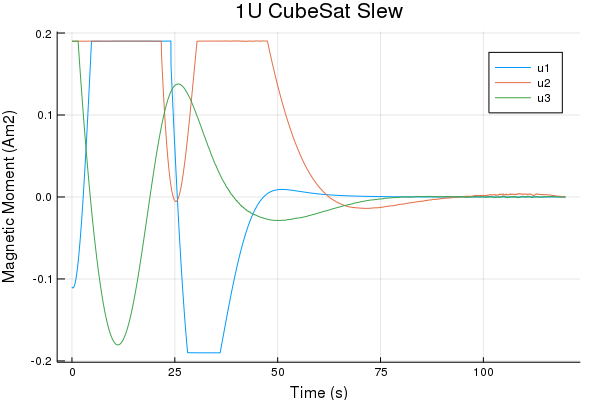
\includegraphics[width=3in]{Figures/1U_control.png} &
	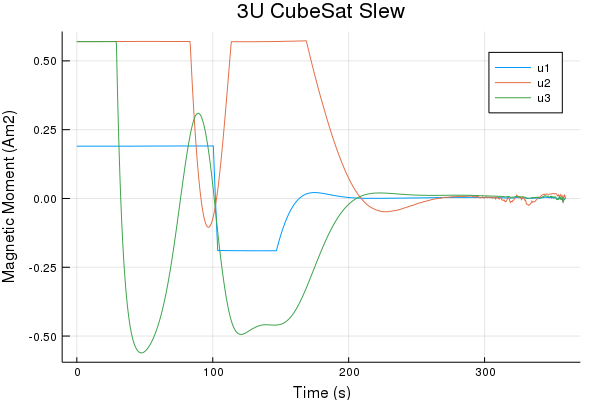
\includegraphics[width=3in]{Figures/3U_control.png}\\
		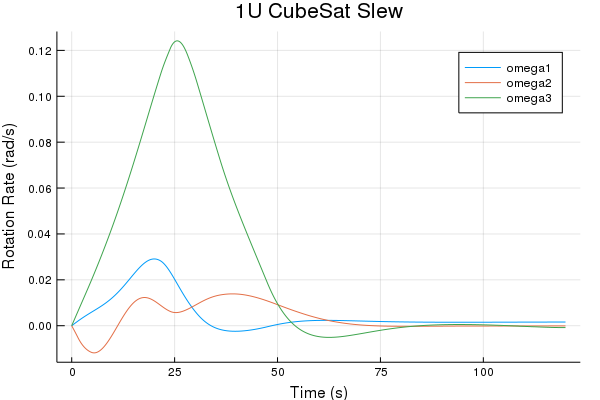
\includegraphics[width=3in]{Figures/1U_rotation.png} &
	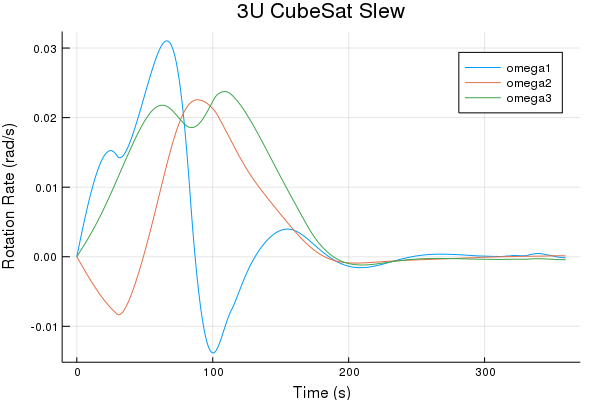
\includegraphics[width=3in]{Figures/3U_rotation.png}\\
	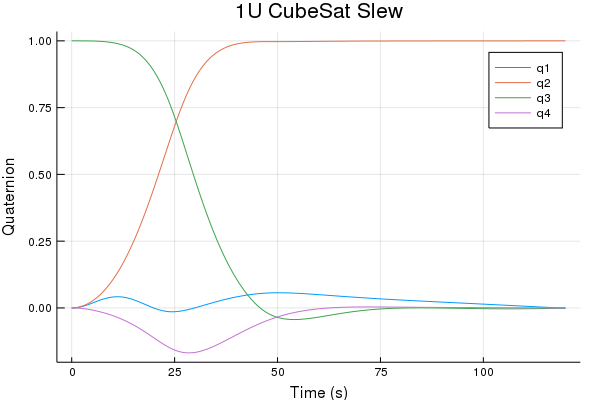
\includegraphics[width=3in]{Figures/1U_quat.png} &
	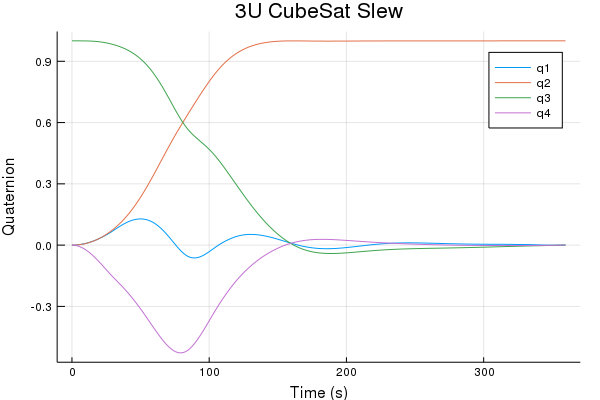
\includegraphics[width=3in]{Figures/3U_quat.png}\\
	\end{array}$
\end{center}
\caption{Simulation Results}
\label{fig:xxx}
\end{figure}

\subsection{1U Monte Carlo}
Since the ability of the CubeSat to rotate is highly dependent on the changing magnetic field, corner cases are a significant concern. Out of any low earth orbit, a circular equatorial orbit experiences the slowest change in magnetic field direction, but equatorial cases showed only minor deterioration in slew time. To ensure that there were no orbits in which the trajectory optimization method broke down, 50 different circular orbits with altitudes of 400 km were tested. The inclination, the right ascension of the ascending node, and the mean anomaly of the starting position were all randomized. The satellite was judged to have finished rotating when:
\begin{equation}
	\label{eq:x}
	||\mathbf{\omega}|| \leq 0.01 \frac{rad}{s}
\end{equation}
for at least 1.8 seconds. Over the 50 different orbits, the mean slew time was found to be 100.2 seconds. The runs with the longest slew times were compared against their magnetic fields, and a general correlation was found between slew time and magnetic field dynanism. The more that the magnetic field vector changed over the course of the simulation, the faster the satellite was able to slew its attitude, as expected. 

\section{Conclusion}
Magnetorquer-only control systems, though underactuated, provide significant promise for small satellite systems. As the size of the satellite shrinks, the control authority of magnetorquers increases significantly due to the scaling of the satellite physical properties. Magnetorquer-based control systems also occupy significantly less volume in a satellite and avoid the jitter common to reaction wheel assemblies necessary for fine pointing. By considering the IGRF magnetic field rather than a simplified periodic assumption, a magnetic-field-based control is more effective due to the sharp, local changes in magnetic field vector. Additionally, as the on-board processing power of small satellites continues to increase with the adoption of careful COTS techniques, powerful trajectory optimization techniques become increasingly feasible without groundstation communication. 

In order to validate and assess the strength of magnetorquer-only control systems for CubeSat specification small satellites, a constrained optimization technique was employed to arrive at an optimal magnetic moment control input. This optimization was composed of an inner loop running iterative LQR and an outer loop updating with augmented lagrangians. The optimal trajectory was then simulated against nominal sensor noise using a time-varying LQR feedback controller. The magnetorquers were shown to actuate the CubeSats quickly and effectively independently of satellite location and orbital parameters, proving the ability of magnetic-field-based control systems to successfully control a CubeSat mission. 

This technology has major applications to the use of CubeSats for missions requiring fine pointing accuracies and rapid slew maneuvers. Even with significant sensor error, the time varying LQR feedback controller was able to maintain accuracy. Due to their small size, it is extremely rare for 1U CubeSats to have a dedicated reaction wheel system, so magnetorquers provide a lightweight, powerful alternative for accurate pointing and maneuvering. 3U CubeSats can also benefit from magnetic-field-based control systems, especially to facilitate fine pointing control for observation without the jitter of reaction wheels. 

Future work will consist of implementing this control system in a flight-ready microcontroller to test computational efficiency on-orbit. The algorithm will be tested against known magnetic field measurements in a hardware-in-the-loop system to validate its ability to provide control trajectories in real time.  

\section{Acknowledgements}
I would like to thank my research advisor, Zac Manchester, for his personal and academic mentorship, without which this project would not be possible.  

\bibliographystyle{AAS_publication}   % Number the references.
\bibliography{references}   % Use references.bib to resolve the labels.

\end{document}
